\noindent
\begin{minipage}[t]{0.26\textwidth}
    % Trang trí 5 vạch ngang màu cyan ở đầu trang lề trái
    \vspace*{4pt}
    \begin{minipage}{\linewidth}
        {\color{stewartcyan}\rule{\linewidth}{0.65pt}}\\[3.2pt]
        {\color{stewartcyan}\rule{\linewidth}{0.65pt}}\\[3.2pt]
        {\color{stewartcyan}\rule{\linewidth}{0.65pt}}\\[3.2pt]
        {\color{stewartcyan}\rule{\linewidth}{0.65pt}}\\[3.2pt]
        {\color{stewartcyan}\rule{\linewidth}{0.65pt}}
    \end{minipage}

    % Dóng hàng với đoạn "Trước khi phát biểu Quy tắc nhân..."
    \vspace*{4.8cm}

    \noindent
    \centering
    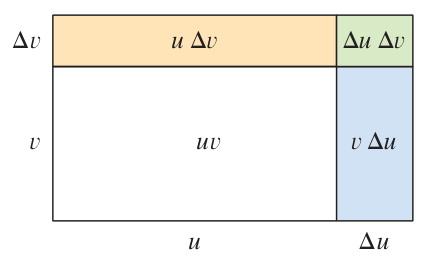
\includegraphics[width=\linewidth]{images/p0220_fig1.png}
    \vspace{4pt}
    
    \raggedright
    \noindent\textbf{\textsf{HÌNH 1}}\\[2pt]
    {\small\textsf{Ý nghĩa hình học của Quy tắc nhân}}

    % Dóng hàng với công thức giới hạn đạo hàm d/dx(uv)
    \vspace{3.2cm}

    \noindent
    {\small\textsf{Nhắc lại rằng trong ký hiệu Leibniz, định nghĩa của đạo hàm có thể được viết dưới dạng}}
    \[
    \frac{dy}{dx} = \lim_{\Delta x \to 0} \frac{\Delta y}{\Delta x}
    \]

    % Dóng hàng với khung Quy tắc nhân ở cuối trang
    \vspace{3.8cm}

    \noindent
    {\small\textsf{Dưới dạng ký hiệu dấu phẩy, Quy tắc nhân được viết là}}
    \[
    (fg)' = fg' + gf'
    \]
\end{minipage}%
\hfill
\begin{minipage}[t]{0.71\textwidth}
    % Tiêu đề mục 3.2
    \noindent
    {\Huge\bfseries\color{stewartcyan}3.2}\;\;{\color{stewartcyan}\vrule width 1.5pt height 22pt depth 4pt}\;\;{\LARGE\bfseries\textsf{Quy tắc nhân và quy tắc thương}}
    \vspace{10pt}

    Các công thức trong mục này cho phép chúng ta tính đạo hàm của các hàm số mới được tạo thành từ các hàm số đã biết bằng phép nhân hoặc phép chia.

    \vspace{4pt}
    \noindent
    {\color{stewartcyan}\rule[0.1ex]{1.1ex}{1.1ex}}\hspace{6pt}\textbf{\large\textsf{Quy tắc nhân}}

    Tương tự như Quy tắc tổng và hiệu, chúng ta có thể có xu hướng phỏng đoán rằng, như Leibniz đã từng nghĩ cách đây ba thế kỷ, đạo hàm của một tích bằng tích các đạo hàm. Tuy nhiên, chúng ta có thể thấy rằng phỏng đoán này là sai lầm qua một ví dụ cụ thể. Xét $f(x) = x$ và $g(x) = x^2$. Khi đó Quy tắc lũy thừa cho ta $f'(x) = 1$ và $g'(x) = 2x$. 
    \llap{\tikz[baseline=-0.6ex]{\draw[thick, stewartred] (0,0) circle (1.1ex); \draw[thick, stewartred] (-0.78ex,0.78ex) -- (0.78ex,-0.78ex);}\hspace{6pt}}%
    Nhưng $(fg)(x) = x^3$, do đó $(fg)'(x) = 3x^2$. Như vậy {\color{stewartred}$(fg)' \neq f'g'$}. Công thức chính xác đã được Leibniz tìm ra (ngay sau bước khởi đầu sai lầm của ông) và được gọi là Quy tắc nhân.

    Trước khi phát biểu Quy tắc nhân, hãy xem làm thế nào chúng ta có thể khám phá ra nó. Ta bắt đầu bằng cách giả sử $u = f(x)$ và $v = g(x)$ đều là các hàm khả vi và nhận giá trị dương. Khi đó, ta có thể hiểu tích $uv$ là diện tích của một hình chữ nhật (xem Hình 1). Nếu $x$ thay đổi một lượng $\Delta x$, thì các lượng thay đổi tương ứng của $u$ và $v$ là
    \[
    \Delta u = f(x + \Delta x) - f(x) \qquad \Delta v = g(x + \Delta x) - g(x)
    \]
    và giá trị mới của tích, $(u + \Delta u)(v + \Delta v)$, có thể xem là diện tích của hình chữ nhật lớn trong Hình 1 (với điều kiện $\Delta u$ và $\Delta v$ đều nhận giá trị dương).

    Độ thay đổi diện tích của hình chữ nhật là
    \begin{align}
    \Delta(uv) &= (u + \Delta u)(v + \Delta v) - uv = u\,\Delta v + v\,\Delta u + \Delta u\,\Delta v \tag*{\fboxsep=2.5pt\fcolorbox{stewartred}{white}{\bfseries\color{stewartred}1}} \\
    &= \text{tổng diện tích của ba phần được tô màu} \notag
    \end{align}

    Nếu chia cho $\Delta x$, ta được
    \[
    \frac{\Delta(uv)}{\Delta x} = u\,\frac{\Delta v}{\Delta x} + v\,\frac{\Delta u}{\Delta x} + \Delta u\,\frac{\Delta v}{\Delta x}
    \]

    Nếu bây giờ ta cho $\Delta x \to 0$, ta nhận được đạo hàm của $uv$:
    \begin{align*}
    \frac{d}{dx}(uv) &= \lim_{\Delta x \to 0} \frac{\Delta(uv)}{\Delta x} = \lim_{\Delta x \to 0} \left( u\,\frac{\Delta v}{\Delta x} + v\,\frac{\Delta u}{\Delta x} + \Delta u\,\frac{\Delta v}{\Delta x} \right) \\[6pt]
    &= u \lim_{\Delta x \to 0} \frac{\Delta v}{\Delta x} + v \lim_{\Delta x \to 0} \frac{\Delta u}{\Delta x} + \left( \lim_{\Delta x \to 0} \Delta u \right) \left( \lim_{\Delta x \to 0} \frac{\Delta v}{\Delta x} \right) \\[6pt]
    &= u\,\frac{dv}{dx} + v\,\frac{du}{dx} + 0 \cdot \frac{dv}{dx}
    \end{align*}
    \begin{equation}
    \frac{d}{dx}(uv) = u\,\frac{dv}{dx} + v\,\frac{du}{dx} \tag*{\fboxsep=2.5pt\fcolorbox{stewartred}{white}{\bfseries\color{stewartred}2}}
    \end{equation}

    (Lưu ý rằng $\Delta u \to 0$ khi $\Delta x \to 0$ vì $f$ khả vi và do đó liên tục.)

    Mặc dù ban đầu chúng ta đã giả thiết (để giải thích bằng hình học) rằng tất cả các đại lượng đều dương, nhưng ta thấy rằng Phương trình 1 luôn đúng. (Các phép biến đổi đại số đều có hiệu lực bất kể $u$, $v$, $\Delta u$ và $\Delta v$ là dương hay âm.) Vì vậy, chúng ta đã chứng minh được Phương trình 2, được gọi là Quy tắc nhân, cho mọi hàm khả vi $u$ và $v$.

    \begin{definitionbox}
    \noindent\textbf{\textsf{\color{stewartred}Quy tắc nhân}}\quad \textsf{Nếu $f$ và $g$ đều khả vi, thì}
    \[
    \frac{d}{dx} [f(x)g(x)] = f(x)\,\frac{d}{dx} [g(x)] + g(x)\,\frac{d}{dx} [f(x)]
    \]
    \end{definitionbox}
\end{minipage}

\vfill
{\tiny\color{stewartgray}\noindent Copyright 2021 Cengage Learning. Mọi quyền được bảo lưu. Không được sao chép, quét hoặc nhân bản toàn bộ hoặc một phần.}
